% This file should contain a short summary of the aerodynamic analysis tool and models

% Summarize the physics
To model the aerostructural performance of the wing, we use OpenAeroStruct, which is an open-source tool for low-fidelity conceptual design of aircraft wings~\cite{Jasa2018a}.
OpenAeroStruct uses a vortex lattice method coupled with a six degree-of-freedom finite element method to analyze the aerostructural properties of aircraft wings.
These low-fidelity methods enable inexpensive exploration of the wing design space.
OpenAeroStruct can be used to investigate both conventional and non-conventional wings because the physics-based analyses do not rely on previously-gathered information from existing planes.
Additionally, OpenAeroStruct provides analytic derivatives for all outputs of the aerostructural analyses, which enables low cost gradient-based optimization.

% Describe the model used by this tool that was developed for the tiltwing plane
Here we use information from Johnson et al's paper, with these values specifically:
Put in table of wing design values and assumptions used
We use point masses for the engine and propellers, which was partially developed for this work

% Describe the inputs and outputs of the model and how it talks to other portions for both static and dynamic
We do both static and dynamic analysis
For static, we do a 3-point aerostructural analysis where we ensure that the wing won't fail
We choose the conditions by doing V-n analysis (cite Raymer) to determine the limiting loads of the aircraft
Include a V-n plot for a nominal flight condition

In the dynamic analysis, we only use an aerodynamic-only analysis
This is because the structural loads in the multipoint case are much more limiting
Nominally, in a regular mission, we will not come close to the structural limit of the aircraft wings
We pass the structural deformation from the 1g case to the aerodynamic cases in the dynamic analysis to get a realistically-deformed wing

\begin{figure}
\begin{center}
 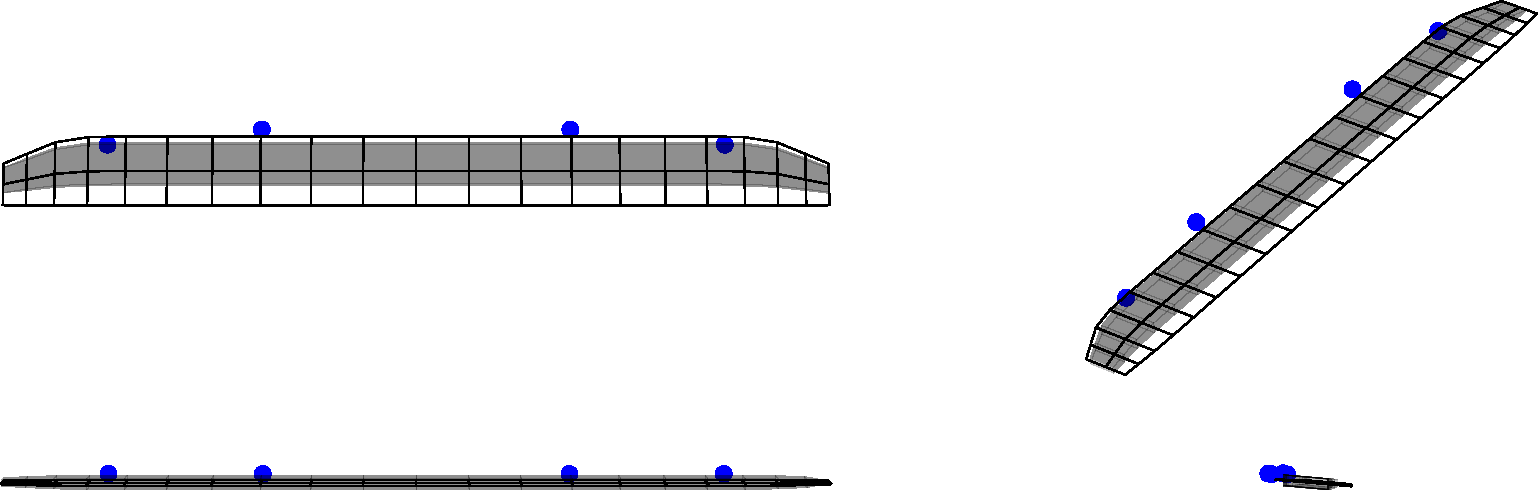
\includegraphics[width=1.0\textwidth]{../Images/aerostruct_wing}
 \caption{Isometric view of the aerostructural wing model with the engine point masses shown in blue.}
 \label{f:OAS_wing}
\end{center}
\end{figure}

\begin{figure}
\begin{center}
 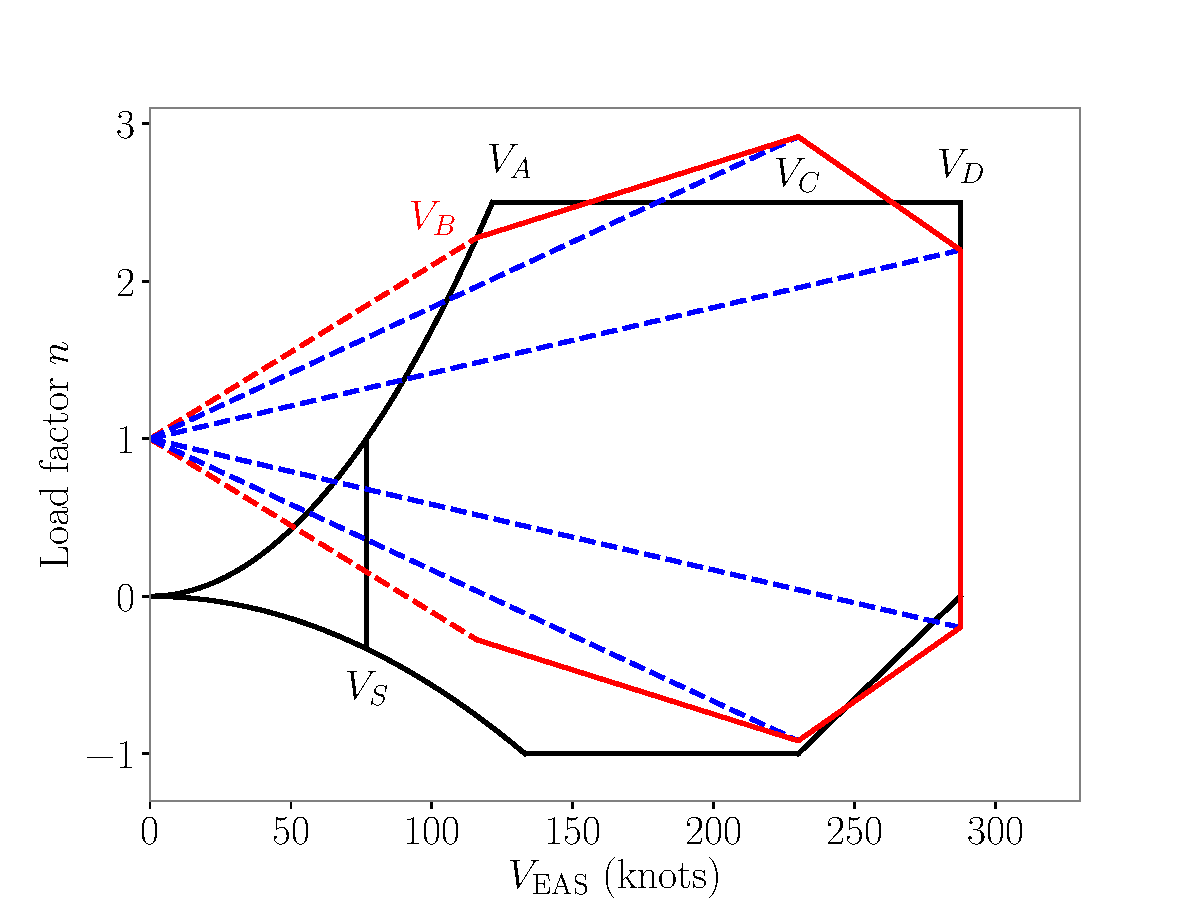
\includegraphics[width=0.7\textwidth]{../Images/v_n_diagram}
 \caption{V-n diagram used to determine the limiting flight conditions for the wing structure.}
 \label{f:v_n_diagram}
\end{center}
\end{figure}
